% !TEX root = SegwayDoku.tex
\renewcommand{\autoren}{Valentyn Chepil, Alexsander Stoiljkovic}
\newpage
\section{Die Gehäuse}
\subsection{Die Gehäusen - V.1}
% \ref{bild_3} zuweisung auf Bild in Text.

\begin{figure}[!h]  % [h] bedeutet, dass das Bild genau an dieser Stelle im Text erscheint
	% mit width=... wird die Größe des Bildes in Prozent der Seitenbreite eingestellt
	\centering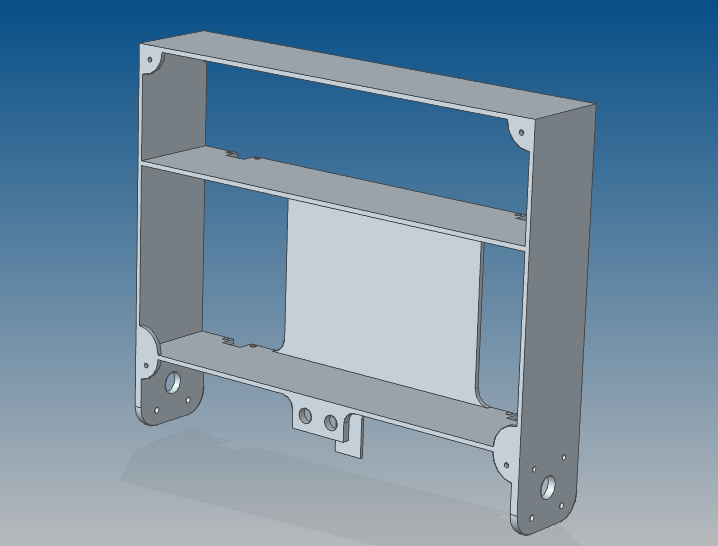
\includegraphics[width=0.5\textwidth]{images/gehaeuse-v1.png}
	% caption ist die Bildunterschrift, taucht auch im Abbildungsverzeichnis auf
	\caption{Gehäuse - V.1 \newline (Quelle: eigene Darstellung)}
	\label{gehaeuse-v1} % über das label kann man aus dem Text auf das Bild verweisen
\end{figure}

\subsection{Die Gehäusen - V.2}
Modul Aufbau: ....
% Text einfügen, dass Herr Nitsche zuerst einfache Gehäuser wollte, danach kam vorschlag Mogulaufbau machen.

\begin{figure}[!h]  % [h] bedeutet, dass das Bild genau an dieser Stelle im Text erscheint
	% mit width=... wird die Größe des Bildes in Prozent der Seitenbreite eingestellt
	\centering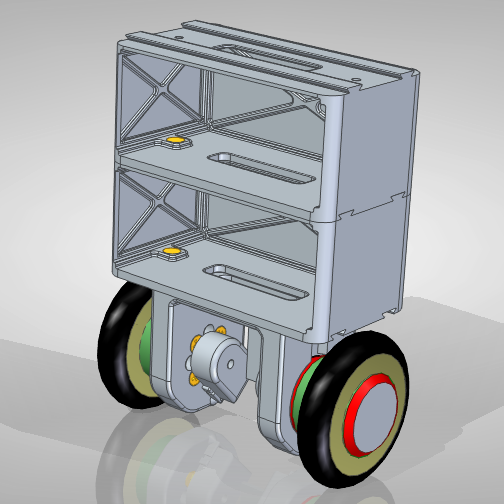
\includegraphics[width=0.5\textwidth]{images/gehaeuse-v2.png}
	% caption ist die Bildunterschrift, taucht auch im Abbildungsverzeichnis auf
	\caption{Gehäuse - V.2 \newline (Quelle: eigene Darstellung)}
	\label{gehaeuse-v2} % über das label kann man aus dem Text auf das Bild verweisen
\end{figure}


Modul, Motorhalter Ansichten zeigen und Text.
\renewcommand{\autoren}{Valentyn Chepil}
\newpage

\subsection{Die Gehäusen - V.3}

Modul Aufbau: ....

% Text einfügen, dass nach lange Beschprechungs mit Herr Nitsche kam eune endgültige Gehäuser.

\begin{figure}[!h]  % [h] bedeutet, dass das Bild genau an dieser Stelle im Text erscheint
	% mit width=... wird die Größe des Bildes in Prozent der Seitenbreite eingestellt
	\centering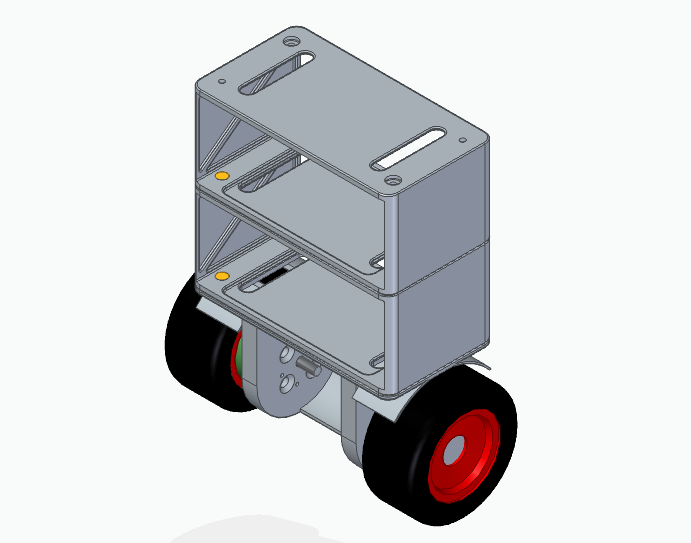
\includegraphics[width=0.5\textwidth]{images/gehaeuse-v3.png}
	% caption ist die Bildunterschrift, taucht auch im Abbildungsverzeichnis auf
	\caption{Gehäuse - V.2 \newline (Quelle: eigene Darstellung)}
	\label{gehaeuse-v3} % über das label kann man aus dem Text auf das Bild verweisen
\end{figure}

\subsubsection{ Berechnung vom Motorhalter}

Alle Berechnungen wurden mit Hilfe von FEM - Programmierung gemacht und beweise die Festigkeit nur von dem Motorhalter. Es wurden an den Stellen vom Motoren und Räder das Moment laut der Berechnung %\ref{ber}
 verwendet und als Lastkraft wurde 50N auf die Oberfläche eingeprägt.

Bild einfügen mit %\ref{ber}

Die Materialeigenschaften kann man auf der Abbildung \ref{FEM2}

\begin{figure}[!h]  % [h] bedeutet, dass das Bild genau an dieser Stelle im Text erscheint
	\centering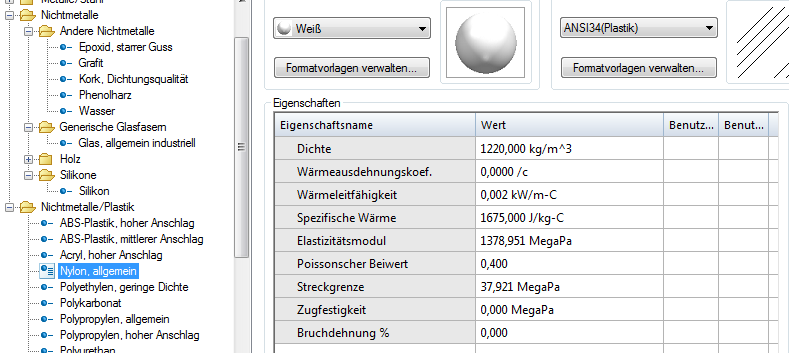
\includegraphics[width=0.7\textwidth]{images/FEM2.png}
	% caption ist die Bildunterschrift, taucht auch im Abbildungsverzeichnis auf
	\caption{Kunststoffeigenschaften - Nylon (PA) \newline (Quelle: eigene Darstellung)}
	\label{FEM2} % über das label kann man aus dem Text auf das Bild verweisen
\end{figure}

\begin{figure}[!h]  % [h] bedeutet, dass das Bild genau an dieser Stelle im Text erscheint
	% mit width=... wird die Größe des Bildes in Prozent der Seitenbreite eingestellt
	\centering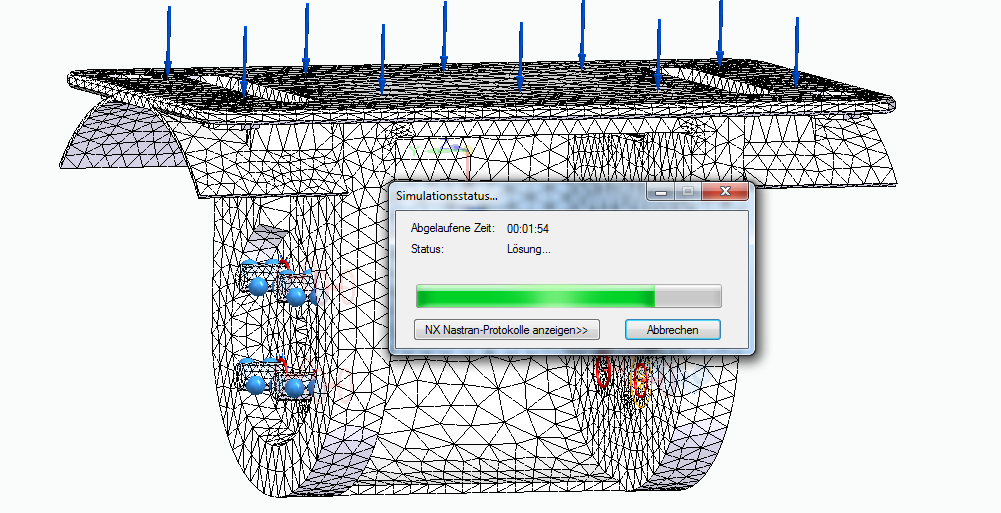
\includegraphics[width=0.9\textwidth]{images/FEM.png}
	% caption ist die Bildunterschrift, taucht auch im Abbildungsverzeichnis auf
	\caption{FEM-Berechnung \newline (Quelle: eigene Darstellung)}
	\label{FEM1} % über das label kann man aus dem Text auf das Bild verweisen
\end{figure}



\begin{figure}[!h]  % [h] bedeutet, dass das Bild genau an dieser Stelle im Text erscheint
	\centering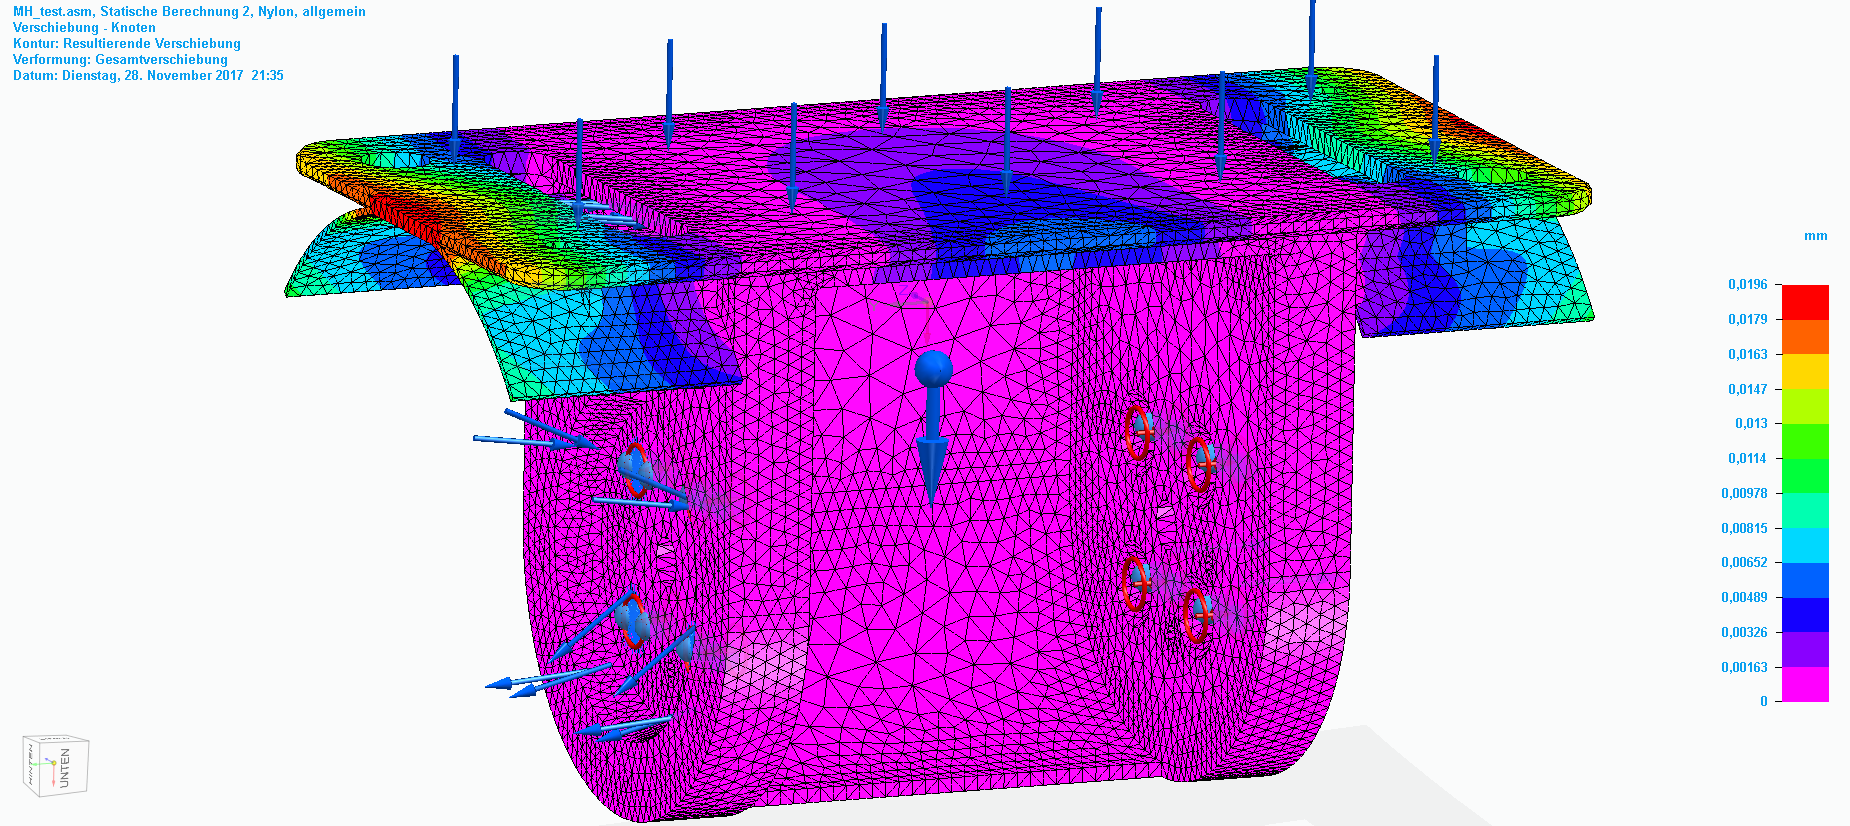
\includegraphics[width=0.9\textwidth]{images/FEM3.png}
	% caption ist die Bildunterschrift, taucht auch im Abbildungsverzeichnis auf
	\caption{FEM - Verschiebungen \newline (Quelle: eigene Darstellung)}
	\label{FEM3} % über das label kann man aus dem Text auf das Bild verweisen
\end{figure}
\begin{figure}[!h]  % [h] bedeutet, dass das Bild genau an dieser Stelle im Text erscheint
	\centering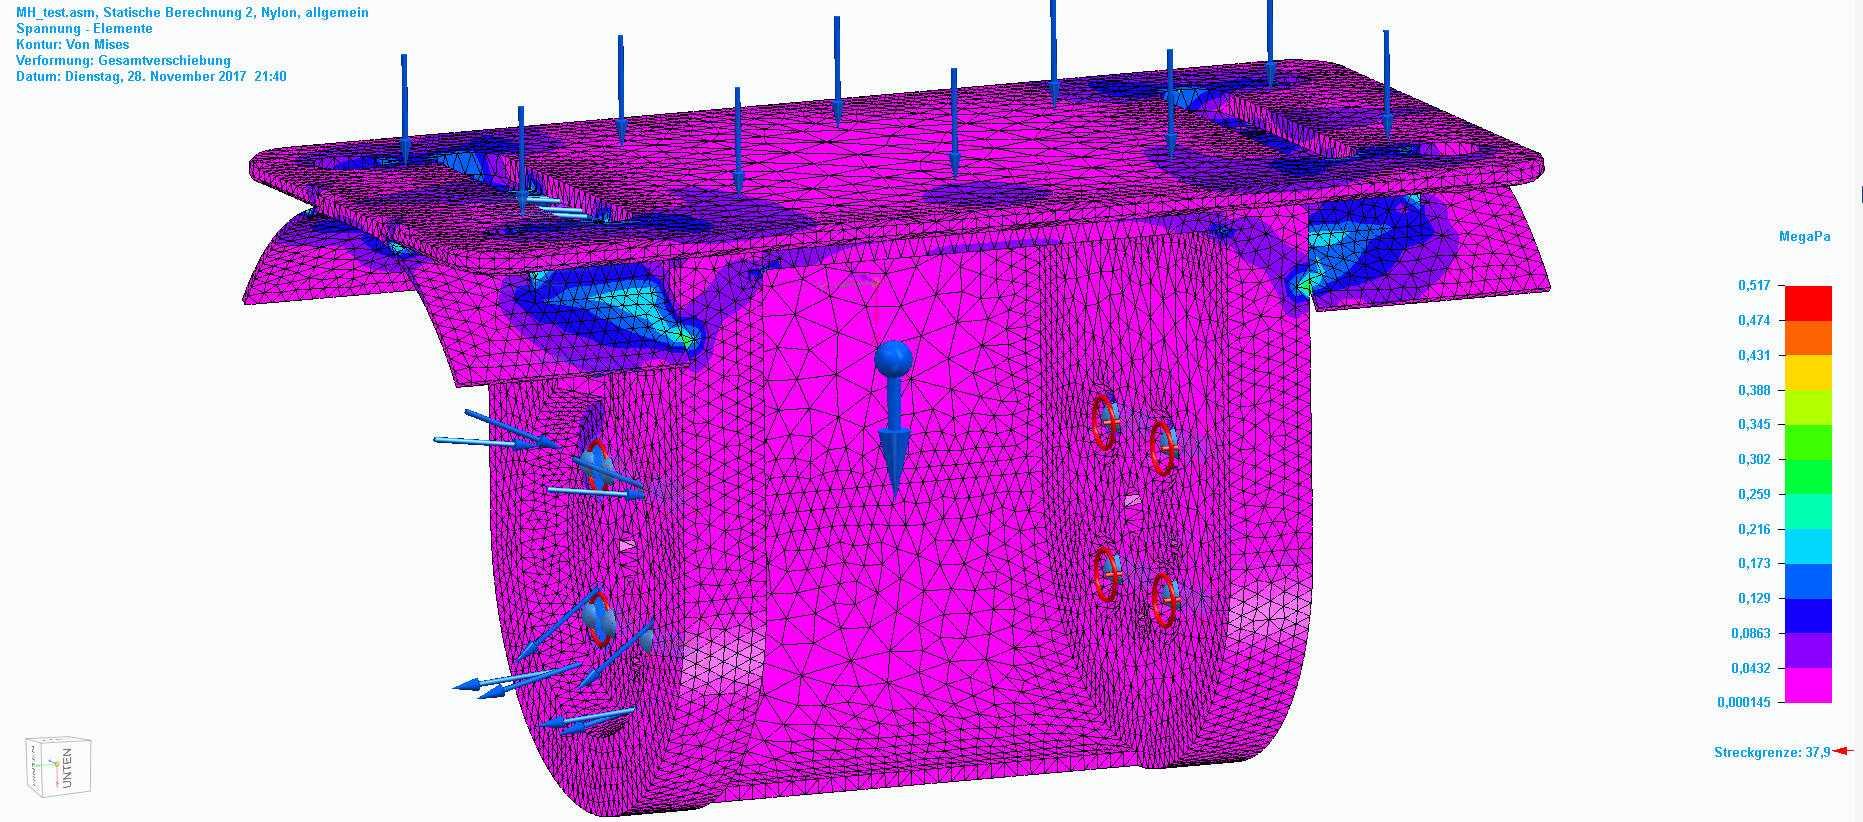
\includegraphics[width=0.9\textwidth]{images/FEM4.png}
	% caption ist die Bildunterschrift, taucht auch im Abbildungsverzeichnis auf
	\caption{FEM - Spannungen \newline (Quelle: eigene Darstellung)}
	\label{FEM4} % über das label kann man aus dem Text auf das Bild verweisen
\end{figure}








\newpage
